\documentclass[11pt,a4paper]{article}

% Packages
\usepackage[utf8]{inputenc}
\usepackage[spanish, es-tabla]{babel}
\usepackage{caption}
\usepackage{listings}
\usepackage{adjustbox}
\usepackage{enumitem}
\usepackage{boldline}
\usepackage{amssymb, amsmath}
\usepackage[margin=1in]{geometry}
\usepackage{xcolor}
%\usepackage{soul}
\usepackage{enumerate}
\usepackage{hyperref}
\usepackage{graphics, graphicx, float}

% Meta
\title{Problema de Máxima Diversidad (MDP) 
	\\\medskip \large Técnicas de búsqueda local y algoritmos greedy \\\medskip
	\large Metaheurísticas: Práctica 1, Grupo 1}
\author{José Antonio Álvarez Ocete - 77553417Q \\ joseantonioao@correo.ugr.es}
\date{ \today }

% Custom
\providecommand{\abs}[1]{\lvert#1\rvert}
\setlength\parindent{0pt}
\definecolor{Light}{gray}{.90}
\newcommand\ddfrac[2]{\frac{\displaystyle #1}{\displaystyle #2}}
\setlength{\parindent}{1.5em} %sangria

% Displaying code with lstlisting
\lstset { %
	language=C++,
	backgroundcolor=\color{black!5}, % set backgroundcolor
	basicstyle=\footnotesize,% basic font setting
}

\usepackage[ruled]{algorithm2e}


\begin{document}	
	
	\maketitle 
	\newpage
	\tableofcontents
	\newpage
	
	
	\section{El problema}
	
	\subsection{Descripción del problema}
	
	El \textbf{problema de la máxima diversidad} (en inglés, \emph{maximum diversity problem}, MDP) es un problema de optimización combinatoria que consiste en seleccionar un
	subconjunto $M$ de $m$ elementos ($|M|=m$) de un conjunto inicial $N$ de $n$ elementos (con $n>m$) de forma que se maximice la diversidad entre los elementos escogidos. El MDP se puede formular como:
	
	$$ \text{Maximizar } z_{MS}(x) = \sum_{i=1}^{n-1} \sum_{j=i+1}^{n} d_{ij} \cdot x_i \cdot x_j $$
	$$ \text{Sujeto a } \sum_{i=1}^{n} x_i = m $$
	$$ x_i \in \{0,1\}, \forall i \in \{1,\dotsc,n\} $$
	
	Donde:
	\begin{itemize}
		\item $x$ es una solución al problema que consiste en un vector binario que indica los $m$ elementos seleccionados.
		\item $d_{ij}$ es la distancia existente entre los elementos $i$ y $j$.
		
	\end{itemize}

	\subsection{Casos considerados}
	
	Se utilizarán 30 casos seleccionados de varios de los conjuntos de instancias disponibles en la \emph{MDPLIB} (\url{http://www.optsicom.es/mdp/}), 10 pertenecientes al grupo \textbf{GKD} con distancias Euclideas, $n=500$ y $m=50$ ($GKD-c\_i\_n500\_m50$ para $i\in\{1,\dotsc,10\}$), 10 del grupo \textbf{SOM} con distancias enteras entre 0 y 999, $n\in\{300,400,500\}$ y $m=\in\{40,\dotsc,200\}$ ($SOM-b\_11\_n300\_m90$ a $SOM-b\_20\_n500\_m200$) y 10 del grupo \textbf{MDG} con distancias enteras entre 0 y 10, $n=2000$ y $m=200$ ($MDG-a\_i\_n2000\_m200$ para $i\in\{21,\dotsc,30\}$. \\
	
	Puesto que la numeración utilizada es unívoca se hará referencia a estas entradas simplemente como \textbf{MDP-a\_i} con $i\in\{1,\dotsc,10\}$, \textbf{SOM-b\_i} con $i\in\{11,\dotsc,20\}$ y \textbf{GKD-c\_i} con $i\in\{21,\dotsc,30\}$.
	
	\section{Descripción de la aplicación de los algoritmos}
	
	En esta sección describiremos las consideraciones comunes a los distintos algoritmos. Este incluye la representación de las soluciones, la función objetivo y los operadores comunes a los distintos algoritmos. Ya que los únicos puntos en común de la búsqueda local y la técnica greedy son la función objetivo y la representación de las soluciones no estudiaremos ningún operador común. Tampoco se han incluido los detalles específicos de un algoritmo a pesar de que sean comunes a varios algoritmos finales, ya que estos son pequeñas variaciones unos y otros.  \\
	
	El lenguaje utilizado para la implementación de la práctica ha sido $C++$. 
	
	\subsection{Representación de la soluciones}
	
	El esquema de representación de una solución es el siguiente:

	\begin{lstlisting}
	struct solution {
		vector<int> v;
		double fitness;
	};
	\end{lstlisting}
	
	Donde el vector contiene números entre $1$ y $n$ no repetidos que componen la solución ( $|v| = m$). Aunque el orden de estos elementos no es relevante se utilizará determinado ordenamiento sobre este mismo vector en algunas de las soluciones planteadas. \\
	
	Cabe destacar que los datos proporcionados únicamente representan las distancias punto a punto, para todos los puntos. Sin embargo se desconoce la posición exacta de cada elemento. Es por esto por lo que no se ha podido implementar la técnica Greedy planteada inicialmente ya que se centraba en el concepto de $centroide$ o $baricentro$ de un conjunto y no podíamos calcularlo sin estimar primero la posición de los puntos. \\
	
	Estos datos se han almacenado en una matriz simétrica de tamaño $n$ x $n$ que de aquí en adelante denotaremos por $MAT$.
	
	\subsection{Función objetivo}
	
	Para la función objetivo se ha dividido la implementación en dos funciones ya que algunos algoritmos utilizarán unicamente una de las dos y otros, ambas. La primera calcula la contribución del elemento $i$ a la solución actual. La segunda calcula el $fitness$ total utilizando la función anterior. \\

	\begin{algorithm}
	\caption{singleContribution}
		\KwData{solution : sol , i : int}
		\KwResult{ contribution : double}
		\Begin{
			contribution $\leftarrow$ 0
			
			\ForEach{ $ j \in sol.v$ }{
				contribution $\leftarrow$ contribution + MAT[ i ][ j ]
			}
		}
	\end{algorithm}
			
	\begin{algorithm}
	\caption{evaluateSolution}
		\KwData{solution : sol}
		\KwResult{fitness : double}
		\Begin{
			fitness $\leftarrow$ 0
			
			\ForEach{ $ i \in sol.v$ }{
				fitness $\leftarrow$ fitness + SingleContribution ( sol, i )
			}
			fitness $\leftarrow$ fitness / 2
		}
	\end{algorithm}
	
	\section{Algoritmos}
	
	Para esta práctica se han implementado un total de 4 algoritmos que a continuación describiremos en profundidad. Son los siguientes:
	\begin{itemize}
		\item Greedy
		\item Búsqueda local
		\item Búsqueda local determinista
		\item Búsqueda local con greedy
	\end{itemize}
		
	\subsection{Greedy}
	
	Como ya se ha comentado, la concepción inicial de la práctica era utilizar la idea del $baricentro$. Para ello en cada iteración se calcularía el baricentro de los elementos de la solución y se escogería el punto más alejado a este entre los aún no escogidos. Intentando simular esta estrategia utilizaremos la suma de las distancias al resto de elementos de la solución para cada punto aún no he escogido. \\
	
	En primer lugar se ha implementado una función que, dados dos conjuntos de puntos, $seleccionados$ y $no\_seleccionados$, devuelve el elemento de $no\_seleccionados$ cuya suma de distancias a los elementos de $seleccionados$ es máxima. Para ello utilizamos la función $SingleContribution$ explicado en el apartado anterior, que computa la suma de distancias de un punto a otro conjunto dado. \\ 

	\begin{algorithm}
		\caption{farthestToSel}
		\KwData{selected : $set<int>$ , non\_selected : $set<int>$}
		\KwResult{farthest : i}
		\Begin{
			fitness $\leftarrow$ 0 \\
			max\_sum\_dist $\leftarrow$ 0 \\
			\ForEach{  i $\in$ non\_selected }{
				current\_sum\_dist $\leftarrow$ SingleContribution ( selected , i ) \\
				\If{current\_sum\_dist $>$ max\_sum\_dist}{
					max\_sum\_dist $\leftarrow$ current\_sum\_dist \\
					farthest $\leftarrow$ i
				}
			}
		}
	\end{algorithm}
	
	De cara al algoritmo greedy final necesitaremos inicializar el conjunto de elementos seleccionados con al menos un elemento. Este será el que esté más alejado de todos los demás. Para calcularlo utilizamos una abstracción de la función anterior, donde $selected$ y $non\_selected$ serán ambos el conjunto de todos los puntos posibles: $\{0,1,\dotsc, n\}$. \\
	
	\begin{algorithm}
		\caption{farthestToAll}
		\KwData{ none }
		\KwResult{farthest : i}
		\Begin{
			all\_elements $\leftarrow  \{0,1,\dotsc, n\}$ \\
			farthest $\leftarrow$ farthestToSel( all\_elements, all\_elements )
		}
	\end{algorithm}

	Finalmente presentamos el algoritmo greedy al completo, haciendo uso de las funciones anteriores. \\

	\begin{algorithm}
		\caption{greedy}
		\KwData{ none }
		\KwResult{selected : $set<int>$}
		\Begin{
			non\_selected $\leftarrow  \{0,1,\dotsc, n\}$ \\
			selected $\leftarrow$ \{ farthestToAll() \} \\
			\While{ $|selected| < m$ }{
				farthest $\leftarrow$ farthestToSel(selected, non\_selected) \\
				non\_selected $\leftarrow$ non\_selected $\bigcup$ \{farthest\} \\
				selected $\leftarrow$ selected - \{farthest\}
			}
		}
	\end{algorithm}


	\subsection{Búsqueda local}
	
	Desgranemos la búsqueda local paso por paso. En primer lugar generamos una solución aleatoria que será el punto de partida. En cada iteración exploramos el vecindario hasta encontrar una solución mejor y sustituimos la actual por la encontrada. Repetimos este proceso hasta que la exploración del vecindario no encuentre una solución mejor. \\
	
	\begin{algorithm}
		\caption{localSearch}
		\KwData{ none }
		\KwResult{sol : solution}
		\Begin{
			sol $\leftarrow$ randomSolution() \\
			stop $\leftarrow $ false \\
			\While{ !stop }{
				stop , sol $\leftarrow$ stepInNeighbourhood(sol)
			}
			
		}
	\end{algorithm}

	La exploración del vecindario realizada en la función $stepInNeighbourhood$ tiene dos detalles relevantes a explicar. Por un lado se ha explicado la factorización del movimiento en el vecindario. Esto es, para estudiar si una solución es mejor en vez de calcular la fitness de la nueva solución y compararla con la actual, estudiamos si el intercambio del elemento $i \in sol$ y el elemento $j$ de los no seleccionados tiene una repercusión positiva en la fitness de la solución. Para ello hacemos uso de la función $SingleContribution$ comparando las contribuciones de cada elemento. Si el intercambio merece la pena ($SingleContribution(i,sol) < SingleContribution(j,sol)$) reajustamos la fitness sumandole la diferencia entre ambas. \\
	
	Por otro lado, a la hora de escoger que elementos $i,j$ comparar, seleccionamos un elemento $j$ que aún no esté en la solución de forma aleatoria y comparamos con todos los posibles $i \in sol$. Una pequeña mejora consiste en ordenar los elementos de la solución en función a la contribución que realizan a esta para intentar intercambiar primero los que menos contribuyan. Veamos como está implementada esta ordenación. Por un lado definimos un operador de comparación que trabaje con parejas $<int, double>$. Esto nos permitirá ordenar el vector solución en orden de contribución creciente. \\
	
	\begin{algorithm}
	 	\caption{operator$<$}
	 	\KwData{ p1 : $pair<int,double>$ , p2 : $pair<int,double>$ }
	 	\KwResult{comp : bool}
	 	\Begin{
	 		comp $\leftarrow$ $p1.second < p2.second$
	 	}
	\end{algorithm}

	A continuación reordenamos los elementos de la solución. \\

	\begin{algorithm}
		\caption{orderSolutionByContribution}
		\KwData{ sol : solution }
		\KwResult{ sol : solution }
		\Begin{
			pairs : $vector<pair<int,double>>$ \\
			\ForEach{ $i \in sol.v$ }{
				pairs[ i ].first $\leftarrow$ i \\
				pairs[ i ].second $\leftarrow$ singleContribution(sol.v, i);
			}
			pairs $\leftarrow$ sort(pairs, $operator<$) \\
			\ForEach{ $i \in sol.v$ }{
				sol.v[ i ] $\leftarrow$ pairs[ i ].first 
			}
		}
	\end{algorithm}

	Para acabar presentamos la exploración del vecindario, donde $rand(a,b)$ devuelve un número entero aleatorio en $[a,b)$. Se ordena el vector solución utilizando $orderSolutionByContribution$ y se toman $i \in sol.v$ en orden creciente y $j \notin sol.v$ para el intercambio. Este $j$ se tomará de forma aleatoria y con el objetivo de explotar plenamente la ordenación utilizada generaremos múltiples $j$'s para cada $i$. \\
	
	Según el guión de prácticas hemos de generar hasta $MAX = 50.000$ vecinos (parejas $(i,j)$ en nuestro caso) antes de parar la búsqueda local. Tras varias pruebas he decidido que merece la pena centrarse en el $10\%$ más prometedor de la solución. Llamemos a este porcentaje $percentage\_studied$. \\
	
	Por lo tanto estudiaremos $max_i = percentage\_studied \cdot |sol|$ elementos de la solución y para cada uno generaremos $max\_random = MAX / max\_i$ valores aleatorios distintos, obteniendo un total de $ max\_i \cdot max\_random = max\_i \cdot (MAX / max\_i) = MAX$ elementos en total. \\

	\begin{algorithm}[H]
		\caption{stepInNeighbourhood}
		\KwData{ sol : solution }
		\KwResult{ stop : bool , sol : solution }
		\Begin{
			sol $\leftarrow$ orderSolutionByContribution(sol) \\
			$max\_i \leftarrow percentage\_studied \cdot |sol|$ \\
			$max\_randoms \leftarrow MAX / max\_i$ \\
			stop $\leftarrow$ true \\
			tries $\leftarrow$ 0 \\
			i $\leftarrow$ 0 \\
			\While{ $i < max\_i$ }{
				element\_out $\leftarrow$ sol.v[ i ] \\
				oldContribution $\leftarrow$  singleContribution(sol.v, element\_out) \\
				j $\leftarrow rand(0,m)$ \\
				k $\leftarrow$ 0 \\
				\While{ $k < max\_k$ }{
					\If{ $j \notin sol.v$ }{
						newContribution $\leftarrow singleContribution(sol.v, j) - MAT[ j ][ element\_out ] $ \\
						\If{ $newContribution > oldContribution$ }{
							sol.v[ i ] $\leftarrow$ j \\
							sol.fitness $\leftarrow sol.fitness + newContribution - oldContribution$ \\
							pairs[ i ].first $\leftarrow$ i \\
							sol $\leftarrow$ false \\
							return
						}
						$k \leftarrow k + 1$\\
					}
					j $\leftarrow rand(0,m)$ \\
				}
				$i \leftarrow k + 1$\\
			}
		
		}
	\end{algorithm}

	\subsection{Búsqueda local determinista}
	
	Este algoritmo esta basado en la búsqueda local recién explicada pero con una pequeña mejora. A la hora de explorar el vecindario también ordenaremos los elementos no seleccionados en función de los más prometedores. Para ello utilizamos la función $obtainBestOrdering$. \\
	
	\begin{algorithm}[H]
		\caption{obtainBestOrdering}
		\KwData{ sol : solution }
		\KwResult{ best\_ordering : vector<int> }
		\Begin{
			pairs : $vector<pair<int,double>>$ \\
			\ForEach{ $i \in {0,\dotsc,n}$ }{
				\If{ $i \notin sol.v$}{
					pairs[ i ].first $\leftarrow$ i \\
					pairs[ i ].second $\leftarrow$ singleContribution(sol.v, i);
				}
			}
			pairs $\leftarrow$ sort(pairs, $operator<$) \\
			\For{ $i$ from $|pairs|-1$ to 0 }{
				best\_ordering[ i ] $\leftarrow$ pairs[ i ].first
			}
		}
	\end{algorithm}
	
	Para el algoritmo en si, repetiremos un razonamiento análogo al anterior. Fijado el número de elementos del vecindario a explorar, $MAX$, exploramos un porcentaje $p_i$ de la solución y un porcentaje $p_k$ del ordenamiento generado a partir de la función $obtainBestOrdering$. \\
	
	Recorreremos la solución hasta $max_i = |sol| \cdot p_i$ y los posibles intercambios hasta $max_k = n \cdot p_k$, teniendo en cuenta que:
	
	$$ max_k \cdot max_i = (n \cdot p_k) \cdot (|sol| \cdot p_i) = MAX$$ 
	
	Si damos un valor a $p_i$ podemos calcular $max_i$ y $max_k$ en función del resto de datos: $ max_k = MAX / max_i $. Finalmente tenemos que tener en cuenta la posibilidad de que $max_k$ sea mayor que el tamaño de $best_ordering$ es por esto que tomamos $max_k = min(MAX / max_i , |best_ordering|)$. En ese caso hemos de actualizar $max_i$ a $min(MAX / max_k, |sol|)$ para asegurarnos de que hacemos la $MAX$ exploraciones. \\ 
	
	Este movimiento esta implementado en la función $stepInNeighbourhoodDet$ que a su vez es llamado por el algoritmo final, $localSearchDet$. \\
	
	\begin{algorithm}[H]
		\caption{stepInNeighbourhoodDet}
		\KwData{ sol : solution }
		\KwResult{ stop : bool , sol : solution }
		\Begin{
			sol $\leftarrow$ orderSolutionByContribution(sol) \\
			best\_ordering $\leftarrow$ obtainBestOrdering(sol) \\
			$percent_i \leftarrow 0.1$
			$max_i \leftarrow percent_i \cdot |sol|$ \\
			$max_k \leftarrow min( MAX / max_i, |best\_ordering|)$ \\
			\If{ $max_k == |best\_ordering|$}{
				$max_i \leftarrow min( MAX / max_k, |sol|)$ 
			}
			stop $\leftarrow$ true \\
			i $\leftarrow$ 0 \\
			\While{ $i < max\_i$ }{
				element\_out $\leftarrow$ sol.v[ i ] \\
				oldContribution $\leftarrow$  singleContribution(sol.v, element\_out) \\
				k $\leftarrow$ 0 \\
				\While{ $k < max\_k$ }{
					j $\leftarrow$ best\_ordering[ k ]
					\If{ $j \notin sol.v$ }{
						newContribution $\leftarrow singleContribution(sol.v, j) - MAT[ j ][element\_out] $ \\
						\If{ $newContribution > oldContribution$ }{
							sol.v[ i ] $\leftarrow$ j \\
							sol.fitness $\leftarrow sol.fitness + newContribution - oldContribution$ \\
							pairs[ i ].first $\leftarrow$ i \\
							sol $\leftarrow$ false \\
							return
						}
						$k \leftarrow k + 1$\\
					}
				}
				$i \leftarrow k + 1$\\
			}
		}
	\end{algorithm}
	
	\begin{algorithm}
		\caption{localSearchDet}
		\KwData{ none }
		\KwResult{sol : solution}
		\Begin{
			sol $\leftarrow$ randomSolution() \\
			stop $\leftarrow $ false \\
			\While{ !stop }{
				stop , sol $\leftarrow$ stepInNeighbourhoodDet(sol)
			}
			
		}
	\end{algorithm}
	
	Cabe destacar que este algoritmo no es determinista por completo ya que la solución inicial tomada es puramente aleatoria. Este detalle es importante puesto que por ello merecerá la pena ejecutarlo múltiples veces en vez de una única vez. \\
	
	\subsection{Búsqueda local con greedy}
	
	El último algoritmo presentado es otra mejora a la búsqueda local. Consiste simplemente en tomar como solución inicial la obtenida por el greedy. 
	
	\begin{algorithm}
	\caption{localSearchGreedy}
	\KwData{ none }
	\KwResult{sol : solution}
	\Begin{
		sol $\leftarrow$ greedy() \\
		stop $\leftarrow $ false \\
		\While{ !stop }{
			stop , sol $\leftarrow$ stepInNeighbourhoodDet(sol)
		}
	}
	\end{algorithm}


	\section{Procedimiento de desarrollo}
	
	Todos los algoritmos se han implementado en $C++$ y se encuentran en la carpeta adjunta. El código esta dividido independientes y autosuficientes que contienen cada uno un algoritmos de los explicados anteriormente. Adicionalmente hay dos archivos más para el tratamiento de los datos. \\
	
	Se han implementado también una serie de scripts en $bash$, así como un $makefile$ que permite la automatización de todo el proceso. El $makefile$ tiene esencialmente dos tipos de comandos: $examples<algoritmo>$ y $measure<algoritmo>$, donde $<algoritmo> \in {Greedy, LS, LSD, LGS}$. El primer comando compila y ejecuta $<algoritmo>$ para tres ejemplos, uno de cada set de entrenamiento. El segundo comando ejecuta 200 veces $<algoritmo>$ en cada caso del problema y hace la media de los datos proporcionados para cada uno de los casos. Los datos de salida se almacenan en $output/<algoritmo>.dat$. \\
	
	Finalmente el comando $measureAll$ ejecuta $measure$ sobre todos los algoritmos excepto $greedy$, ya que no tienen ningún componente aleatorio. Para tomar datos sobre el algoritmo $greedy$ ejecutaremos $measureGreedy$ una única vez. \\
	
	Para el experimento 4 se ha utilizado el script $evolution.sh$ modificando ligeramente los fuentes para obtener los datos requeridos. 
	
	\section{Experimentos realizados}
	
	En esta sección describiremos los experimentos realizados y estudiáremos los resultados obtenidos. 
	
	\subsection{Experimentos 1: resultados iniciales}
	
	En primer lugar he tomado datos como se expone en la sección anterior. Adjunto a continuación las tablas de los tiempos y los resultados obtenidos para los cuatro algoritmos mencionados.
	
	\begin{table}[H]
		\begin{tabular}{l|l|l|l|l|l|}
			\cline{2-6}
			& Algoritmo Greedy & Búsqueda Local & BS Determinista & BS y Greedy & Óptimos \\ \hline
			\multicolumn{1}{|l|}{MDG-a\_1}  & 112135           & 105832         & 106473          & 112073      & 114259            \\ \hline
			\multicolumn{1}{|l|}{MDG-a\_2}  & 112109           & 105962         & 106416          & 112219      & 114327            \\ \hline
			\multicolumn{1}{|l|}{MDG-a\_3}  & 112541           & 105776         & 106267          & 112199      & 114123            \\ \hline
			\multicolumn{1}{|l|}{MDG-a\_4}  & 112590           & 105884         & 106318          & 112278      & 114040            \\ \hline
			\multicolumn{1}{|l|}{MDG-a\_5}  & 112204           & 106118         & 106598          & 112684      & 114064            \\ \hline
			\multicolumn{1}{|l|}{MDG-a\_6}  & 112347           & 106099         & 106568          & 111997      & 114204            \\ \hline
			\multicolumn{1}{|l|}{MDG-a\_7}  & 112583           & 105940         & 106446          & 112498      & 114338            \\ \hline
			\multicolumn{1}{|l|}{MDG-a\_8}  & 112023           & 105829         & 106320          & 112214      & 114158            \\ \hline
			\multicolumn{1}{|l|}{MDG-a\_9}  & 112411           & 106290         & 106520          & 112173      & 114132            \\ \hline
			\multicolumn{1}{|l|}{MDG-a\_10} & 112634           & 105981         & 106536          & 112565      & 114197            \\ \hline
			\multicolumn{1}{|l|}{SOM-b\_11} & 20420            & 19181          & 20619.6         & 20447.6     & 20743             \\ \hline
			\multicolumn{1}{|l|}{SOM-b\_12} & 35574            & 33798.3        & 35689.9         & 35381.9     & 35881             \\ \hline
			\multicolumn{1}{|l|}{SOM-b\_13} & 4542             & 3955.94        & 4541.65         & 4466.66     & 4658              \\ \hline
			\multicolumn{1}{|l|}{SOM-b\_14} & 16888            & 15500.5        & 16878.1         & 16644       & 16956             \\ \hline
			\multicolumn{1}{|l|}{SOM-b\_15} & 36065            & 33870.9        & 36259.9         & 35934.8     & 36317             \\ \hline
			\multicolumn{1}{|l|}{SOM-b\_16} & 62294            & 59575.7        & 62722.7         & 62128.6     & 62487             \\ \hline
			\multicolumn{1}{|l|}{SOM-b\_17} & 6938             & 6135.27        & 6991.79         & 6934.05     & 7141              \\ \hline
			\multicolumn{1}{|l|}{SOM-b\_18} & 25843            & 23954.5        & 25826.1         & 25642.2     & 26258             \\ \hline
			\multicolumn{1}{|l|}{SOM-b\_19} & 55406            & 52741.8        & 55894.9         & 55400.2     & 56572             \\ \hline
			\multicolumn{1}{|l|}{SOM-b\_20} & 96593            & 92657.6        & 96398.7         & 96375       & 97344             \\ \hline
			\multicolumn{1}{|l|}{GKD-c\_21} & 17831.8          & 16483          & 18051.3         & 17663.6     & 19485,1875        \\ \hline
			\multicolumn{1}{|l|}{GKD-c\_22} & 17973            & 16797.3        & 18188.1         & 17875.2     & 19701,53711       \\ \hline
			\multicolumn{1}{|l|}{GKD-c\_23} & 17973.3          & 16574.8        & 18036.6         & 17592       & 19547,20703       \\ \hline
			\multicolumn{1}{|l|}{GKD-c\_24} & 17860            & 16384.7        & 18052.7         & 17939.1     & 19596,46875       \\ \hline
			\multicolumn{1}{|l|}{GKD-c\_25} & 17822.9          & 16702.6        & 18013.9         & 17675.1     & 19602,625         \\ \hline
			\multicolumn{1}{|l|}{GKD-c\_26} & 17741.1          & 16505.8        & 17991.6         & 17858.9     & 19421,55078       \\ \hline
			\multicolumn{1}{|l|}{GKD-c\_27} & 18016.5          & 16567.3        & 18161.9         & 17896.4     & 19534,30664       \\ \hline
			\multicolumn{1}{|l|}{GKD-c\_28} & 17897.7          & 16522.3        & 18089.3         & 17900.1     & 19487,32031       \\ \hline
			\multicolumn{1}{|l|}{GKD-c\_29} & 17784.5          & 16374.5        & 17817.6         & 17519.4     & 19221,63477       \\ \hline
			\multicolumn{1}{|l|}{GKD-c\_30} & 17860.1          & 16578          & 18042.7         & 17850.2     & 19703,35156       \\ \hline
		\end{tabular}
		\caption{ Costes }
		\label{costes}
	\end{table}

	
	\begin{table}[H]
		\begin{tabular}{l|l|l|l|l|}
			\cline{2-5}
			& \multicolumn{1}{c|}{Greedy} & \multicolumn{1}{c|}{Búsqueda local} & \multicolumn{1}{c|}{BS determinista} & \multicolumn{1}{c|}{BS greedy} \\ \hline
			\multicolumn{1}{|l|}{MDG-a\_1}  & 0.249346                    & 1.29837                             & 1.67138                              & 0.259307                       \\ \hline
			\multicolumn{1}{|l|}{MDG-a\_2}  & 0.251498                    & 1.25412                             & 1.64122                              & 0.299649                       \\ \hline
			\multicolumn{1}{|l|}{MDG-a\_3}  & 0.25458                     & 1.32799                             & 1.64147                              & 0.281972                       \\ \hline
			\multicolumn{1}{|l|}{MDG-a\_4}  & 0.264134                    & 1.30341                             & 1.66133                              & 0.310694                       \\ \hline
			\multicolumn{1}{|l|}{MDG-a\_5}  & 0.258874                    & 1.30089                             & 1.71872                              & 0.285821                       \\ \hline
			\multicolumn{1}{|l|}{MDG-a\_6}  & 0.259026                    & 1.33751                             & 1.74401                              & 0.334614                       \\ \hline
			\multicolumn{1}{|l|}{MDG-a\_7}  & 0.260951                    & 1.34526                             & 1.69168                              & 0.297083                       \\ \hline
			\multicolumn{1}{|l|}{MDG-a\_8}  & 0.258524                    & 1.35116                             & 1.71162                              & 0.314464                       \\ \hline
			\multicolumn{1}{|l|}{MDG-a\_9}  & 0.257905                    & 1.43386                             & 1.76812                              & 0.259414                       \\ \hline
			\multicolumn{1}{|l|}{MDG-a\_10} & 0.252341                    & 1.3025                              & 1.74672                              & 0.262792                       \\ \hline
			\multicolumn{1}{|l|}{SOM-b\_11} & 0.003922                    & 0.0769007                           & 0.094339                             & 0.0115729                      \\ \hline
			\multicolumn{1}{|l|}{SOM-b\_12} & 0.005933                    & 0.168331                            & 0.178364                             & 0.0135729                      \\ \hline
			\multicolumn{1}{|l|}{SOM-b\_13} & 0.001846                    & 0.0198992                           & 0.0233178                            & 0.00484763                     \\ \hline
			\multicolumn{1}{|l|}{SOM-b\_14} & 0.004533                    & 0.0882583                           & 0.11522                              & 0.010587                       \\ \hline
			\multicolumn{1}{|l|}{SOM-b\_15} & 0.008492                    & 0.189072                            & 0.360455                             & 0.0206853                      \\ \hline
			\multicolumn{1}{|l|}{SOM-b\_16} & 0.013224                    & 0.326374                            & 0.634729                             & 0.0254535                      \\ \hline
			\multicolumn{1}{|l|}{SOM-b\_17} & 0.003302                    & 0.0304316                           & 0.0500629                            & 0.00627894                     \\ \hline
			\multicolumn{1}{|l|}{SOM-b\_18} & 0.008476                    & 0.126879                            & 0.306938                             & 0.0167809                      \\ \hline
			\multicolumn{1}{|l|}{SOM-b\_19} & 0.016259                    & 0.260259                            & 0.765596                             & 0.071728                       \\ \hline
			\multicolumn{1}{|l|}{SOM-b\_20} & 0.025305                    & 0.456821                            & 1.14616                              & 0.0639032                      \\ \hline
			\multicolumn{1}{|l|}{GKD-c\_21} & 0.003234                    & 0.0399083                           & 0.0699487                            & 0.00735801                     \\ \hline
			\multicolumn{1}{|l|}{GKD-c\_22} & 0.003143                    & 0.0509766                           & 0.0709061                            & 0.00732955                     \\ \hline
			\multicolumn{1}{|l|}{GKD-c\_23} & 0.003172                    & 0.0460402                           & 0.0729913                            & 0.01287                        \\ \hline
			\multicolumn{1}{|l|}{GKD-c\_24} & 0.003158                    & 0.0489642                           & 0.0817394                            & 0.0074404                      \\ \hline
			\multicolumn{1}{|l|}{GKD-c\_25} & 0.003188                    & 0.0501347                           & 0.0702928                            & 0.00716391                     \\ \hline
			\multicolumn{1}{|l|}{GKD-c\_26} & 0.003173                    & 0.0519859                           & 0.0584565                            & 0.00720639                     \\ \hline
			\multicolumn{1}{|l|}{GKD-c\_27} & 0.004301                    & 0.0562678                           & 0.0815131                            & 0.00846629                     \\ \hline
			\multicolumn{1}{|l|}{GKD-c\_28} & 0.003306                    & 0.0476838                           & 0.0648686                            & 0.00651156                     \\ \hline
			\multicolumn{1}{|l|}{GKD-c\_29} & 0.003221                    & 0.0512277                           & 0.0611578                            & 0.00678151                     \\ \hline
			\multicolumn{1}{|l|}{GKD-c\_30} & 0.00325                     & 0.0478213                           & 0.0706898                            & 0.00764579                     \\ \hline
		\end{tabular}
		\caption{ Tiempos (s) }
		\label{tiempos}
	\end{table}

	\begin{table}[H]
		\begin{tabular}{l|l|l|l|l|}
			\cline{2-5}
			& Greedy & Búsqueda Local & BL Determinista & BL con greedy \\ \hline
			\multicolumn{1}{|l|}{Desv}       & 3,81   & 10,25          & 5,12            & 4,17          \\ \hline
			\multicolumn{1}{|l|}{Tiempo (s)} & 0,09   & 0,52           & 0,71            & 0,11          \\ \hline
		\end{tabular}
		\caption{ Comparativa entre algoritmos }
		\label{comparativa}
	\end{table}

	\subsubsection{ Análisis }
	
	Comencemos observando la tabla \ref{comparativa} para obtener una visión general de los datos. Por un lado los tiempos no son para nada sorprendentes: La $BLD$ es el algoritmo más lento seguido de la búsqueda local clásica. Entenderemos mejor el tiempo obtenido para la $BL con greedy$ en los siguientes experimentos. \\
	
	Por otro lado el algoritmo $Greedy$ obtiene un valor $Desv$ menor que los de la búsqueda local. Sin embargo, si miramos la tabla \ref{costes} con más detenimiento nos damos cuenta de que efectivamente sobre los casos $MDG$ el algoritmo $Greedy$ obtiene mejores costes, pero en los demás casos la $BLD$ suele superarlo. Este es un claro ejemplo de como un algoritmo puede ser más efectivo frente a un caso de estudio particular y no serlo en otro. \\ 
	
	En cuanto a la $BL con Greedy$ era de esperar que tuviese valores como mínimo mejores que los del $Greedy$. Observamos que sin embargo estos valores no son notablemente mejores. Surgen por lo tanto dos preguntas: Por qué el tiempo de ejecución de $BL con Greedy$ es tan bajo y por qué su coste apenas mejora respecto al $Greedy$. Ambas preguntas serán contestadas en el segundo experimento. \\
	
	\subsection{ Experimento 2: exploración del vecindario }
	
	Motivado por las anteriores cuestiones he estudiado las iteraciones que toma cada algoritmo de búsqueda local hasta converger. Esto nos permite estudiar por un lado si la $BLD$ merece la pena y por otro comparar la convergencia de forma general. Estos han sido los resultados obtenidos. \\
	
	\begin{table}[H]
		\begin{tabular}{l|l|l|l|}
			\cline{2-4}
			& Búsqueda Local & BS Determinista & BS con greedy \\ \hline
			\multicolumn{1}{|l|}{MDG-a\_1}  & 333.34         & 458.93          & 1.06          \\ \hline
			\multicolumn{1}{|l|}{MDG-a\_2}  & 341.42         & 460.72          & 3.375         \\ \hline
			\multicolumn{1}{|l|}{MDG-a\_3}  & 333.32         & 445.39          & 3.615         \\ \hline
			\multicolumn{1}{|l|}{MDG-a\_4}  & 334.15         & 450.24          & 4.035         \\ \hline
			\multicolumn{1}{|l|}{MDG-a\_5}  & 341.59         & 466.07          & 2.615         \\ \hline
			\multicolumn{1}{|l|}{MDG-a\_6}  & 350.235        & 484.405         & 7.455         \\ \hline
			\multicolumn{1}{|l|}{MDG-a\_7}  & 342.575        & 452.6           & 2.71          \\ \hline
			\multicolumn{1}{|l|}{MDG-a\_8}  & 337.055        & 477.755         & 3.9           \\ \hline
			\multicolumn{1}{|l|}{MDG-a\_9}  & 357.475        & 479.48          & 1.095         \\ \hline
			\multicolumn{1}{|l|}{MDG-a\_10} & 341.795        & 472.395         & 1.195         \\ \hline
			\multicolumn{1}{|l|}{SOM-b\_11} & 77.785         & 371.73          & 1.555         \\ \hline
			\multicolumn{1}{|l|}{SOM-b\_12} & 102.11         & 466.15          & 1             \\ \hline
			\multicolumn{1}{|l|}{SOM-b\_13} & 44.015         & 189.585         & 1.205         \\ \hline
			\multicolumn{1}{|l|}{SOM-b\_14} & 97.2           & 378.75          & 2             \\ \hline
			\multicolumn{1}{|l|}{SOM-b\_15} & 115.06         & 543.42          & 2.495         \\ \hline
			\multicolumn{1}{|l|}{SOM-b\_16} & 143.41         & 674.185         & 2.37          \\ \hline
			\multicolumn{1}{|l|}{SOM-b\_17} & 56.64          & 252.86          & 1.145         \\ \hline
			\multicolumn{1}{|l|}{SOM-b\_18} & 119.47         & 511.075         & 1.57          \\ \hline
			\multicolumn{1}{|l|}{SOM-b\_19} & 145.545        & 720.03          & 12.72         \\ \hline
			\multicolumn{1}{|l|}{SOM-b\_20} & 179.53         & 785.815         & 5.48          \\ \hline
			\multicolumn{1}{|l|}{GKD-c\_21} & 38.005         & 255.305         & 2.28          \\ \hline
			\multicolumn{1}{|l|}{GKD-c\_22} & 48.95          & 281.135         & 2.545         \\ \hline
			\multicolumn{1}{|l|}{GKD-c\_23} & 42.24          & 268.165         & 3.3           \\ \hline
			\multicolumn{1}{|l|}{GKD-c\_24} & 37.6           & 257.63          & 2.265         \\ \hline
			\multicolumn{1}{|l|}{GKD-c\_25} & 50.375         & 281.54          & 2.135         \\ \hline
			\multicolumn{1}{|l|}{GKD-c\_26} & 41.32          & 258.45          & 2.12          \\ \hline
			\multicolumn{1}{|l|}{GKD-c\_27} & 38.74          & 306.75          & 2.495         \\ \hline
			\multicolumn{1}{|l|}{GKD-c\_28} & 42.035         & 259.42          & 2.145         \\ \hline
			\multicolumn{1}{|l|}{GKD-c\_29} & 41.83          & 281.97          & 3.25          \\ \hline
			\multicolumn{1}{|l|}{GKD-c\_30} & 42.225         & 278.765         & 2.565         \\ \hline
		\end{tabular}
		\caption{ Estudio de convergencia (iteraciones) }
		\label{iteraciones}	
	\end{table}
	
	\subsubsection{ Análisis }
	
	Observando los resultados quedan claramente resueltas las cuestiones planteadas inicialmente. La convergencia es terriblemente prematura en el caso de la $BL con Greedy$, y esto explica tanto los bajos valores de tiempos como la reducida mejora en coste respecto al $Greedy$ inicial. Conjeturo que esta convergencia se debe a la cota en el número de vecinos generados impuesto ($50.000$), a la manera de explorar el vecindario y a la calidad de la solución inicial obtenida con el $Greedy$. \\
	
	Por otra parte observamos que el número de iteraciones para la $BLD$ es considerablemente mayor que para la $BL$, llegando hasta a cuadruplicarse en ocasiones, como es el caso de $SOM-b_12$. Esto no indica que los reajustes realizados realmente merecen la pena en cuanto a costes, si bien en tiempo puede que no sea el caso si ejecutamos esta búsqueda de forma reiterada. \\
	
	En vista de estos últimos resultados otra alternativa sería aplicar la $BLD$ con solución inicial la obtenida por el $Greedy$. Este sería un algoritmo 100\% determinista que explotaría al en profundidad el entorno de la solución inicial. \\
	
	En base a los resultados anteriores se plantean un tercer experimento.  \\
	
	\subsection{ Experimento 3: búsqueda del óptimo }
	
	En el primer experimento podíamos observar como en algunos casos del problema obteníamos valores mejores que los óptimos conocidos, como es el caso de $SOMB-b_16$ en la tabla \ref{costes}. Dicha observación propicia el siguiente experimento, en este caso buscando la mejor solución posible. Para ello se han utilizado las tres búsquedas ya explicadas pero eliminando la cota de generación del vecindario.
	
	\subsection{ Experimento 4: estudio evolutivo de la exploración del entorno }
	
	En este último experimento estudiamos la convergencia de la búsqueda local clásica y la determinista iteración a iteración. Para ello ejecutamos estos algoritmos sobre los conjuntos de datos $MDG-a_21$ y $SOM-b_13$, escogidos por tener comportamientos particularmente distintos en las tablas \ref{costes} y \ref{iteraciones}. Volvemos a utilizar la cota en la exploración del vecindario, y en cada iteración obtenemos el coste actual de la solución en estudio. Podemos ver los resultados obtenidos en las siguientes gráficas.
	
	\begin{figure}[H] 
		\centering
		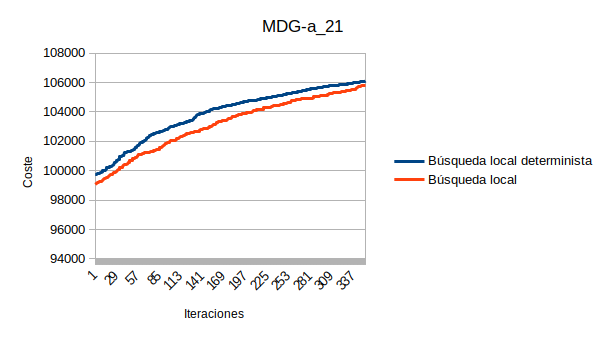
\includegraphics[scale=1]{../output/evolution/MDG-a_21} 
		%\caption{Bomba de prueba - gdb} \label{fig:figura25}
	\end{figure}
	
	\begin{figure}[H] 
		\centering
		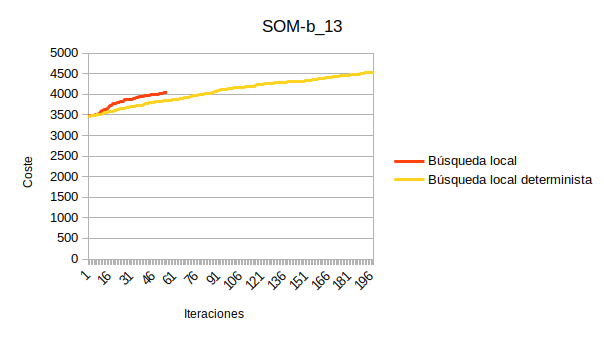
\includegraphics[scale=1]{../output/evolution/SOM-b_13} 
		%\caption{Bomba de prueba - gdb} \label{fig:figura25}
	\end{figure}

	\subsubsection{ Análisis }
	
	Podemos ver como en los distintos casos la evolución es particularmente distinta. Por un lado, para $MDG-a_21$ la convergencia de ambos algoritmos es asintóticamente idéntica, manteniéndose la $BLD$ por encima en parte debido a la solución inicial ligeramente mejor.Por otro, en $SOM-b_13$ la mejora de la $BL$ respecto a la $BLD$ es sustancial pero esta se estanca rápidamente debido a que su exploración del espacio es peor. Este es otro ejemplo de como los mismos algoritmos pueden comportarse de formas completamente distintas para entradas diferentes.

\end{document}